\chapter{Tau Identification Studies}
\label{chap:TauIDStudies}

\noindent Several studies were performed on the tau identification
criteria in order to optimize the signal acceptance 
and to reduce any background contribution. These criteria 
are based on:

\begin{itemize}
 \item the number of prongs (\textit{1or3-prongs} or \textit{1or2or3-prongs}),
 \item the MVA-based isolation discriminator (\textit{loose}, \textit{medium} or \textit{tight}),
 \item the discriminator against electrons (\textit{loose} or \textit{very loose}),
 \item the discriminator against muons (\textit{loose} and \textit{tight}),
 \item the decay mode discriminator (\textit{newDMF} or \textit{oldDMF})
\end{itemize}

\noindent In order to study the impact on the sensitivity due to a particular 
working point (WP), for a  given discriminator, the significance is computed
as a function of the effective visible mass. The significance is defined as $s/\sqrt{s + b}$, where the signal 
yield $s$ and the total background $b$ are estimated using 
the event selection and the background estimation described in 
Chapter \ref{chap:Analysis}. A comparison among the 
significances obtained for each WP is performed in order
determine the optimal selection for each discriminator. The tau 
identification criteria recommended by the TauPOG, which differ from those used 
in this analysis, were considered for these studies. \\

\noindent In this analysis, we select taus with \textit{1or3-prongs}, whose decay 
mode is reconstructed using the \textit{newDMF} discriminator. For the 
MVA-based isolation discriminator the \textit{tight} working point 
was required. Additionally, taus are required to pass the 
the \textit{loose} WP of the discriminator against electrons and the \textit{tight} 
WP for the discrimination against muons. These selection criteria 
are summarized in Table \ref{tab:tauIDappendix}. Besides 
the sensitivity reached in the \Zprimetotauh~channel,
the selection of the working points for the discriminators is 
based on the consistency with the \tauh~identification criteria 
used in the others di-tau channels. 

\begin{table}[H]
    \begin{center}
    \begin{tabular}{l|l} \hline \hline 
 Tau Decay               & \textit{1or3-prongs} \\
                        & \textit{newDMF} \\
 Isolation Disc.        & \textit{by\textbf{Tight}IsolationMVArun2v1DBnewDMwLT} \\
 Anti-electron Disc.    & \textit{againstElectronMVA\textbf{Loose}MVA6} \\
 Anti-muon Disc.        & \textit{againstMuon\textbf{Tight}3} \\ \hline \hline 
  \end{tabular}
  \end{center}
  \caption{Tau Identification Criteria. \label{tab:tauIDappendix}}
\end{table}

% The tau identification criteria depend on several factors, such
% as the number of prongs, the working points of the discriminators
% against QCD-jets, electrons and muons, and the decay mode
% finding algorithm. Since the tau identification criteria are crucial 
% for the sensitivity of this analysis, several studies were performed


\section{Number of prongs Study}
\label{Results:TauID-nprongs}

\noindent The tau identification algorithm considers an 
unphysical 2-prong final state, which can result from 
high-\pt~taus in the 3-prong decay mode. In this case,
due to finite spatial resolution of the Tracker System, two of the 
three tracks can be merged and reconstructed as a single charged 
hadron, resulting in an apparent 2-prong final state. The signal 
and background estimation were performed including this 
unphysical final state in the tau identification criteria (1or2or3-prongs).
Table \ref{tab:prongsappendix} shows the overall yields obtained 
using both selections, 1or3-prongs and 1or2or3-prongs, for the tau 
identification. Note, that the QCD contamination increases considerably for 1or2or3-prongs case, which 
produces a decrease on the sensitivity of the analysis. Figure \ref{fig:prongsappendix} shows 
the significance obtained using both criteria, 1or3-prongs and 1or2or3-prongs. Since a better 
significance is obtained for \mass~$>$ 600 \GeV, where the signal is expected, 
the 1or3-prongs selection was used in this analysis.

% The results are expected since 
% including the 2-prong final state reduces the tau identification efficiency
% for the other decay modes.
% The significance was estimated including this unphysical physical 
% state in the tau identification criteria (1or2or3-prongs). 

 \begin{tiny} 
 \begin{table}[ht] 
 \centering{ 
 \begin{tabular}{ | l | r | r |} \hline \hline 
 \multicolumn{3}{|c|}{OVERALL YIELDS} \\ \hline 
 & 1or3-prongs &  1or2or3-prongs  \\ \hline \hline 
 DY         & 131.61   $\pm$   8.64 & 151.98   $\pm$   9.09 \\ \hline 
 WJets      & 41.91   $\pm$   5.17 & 65.18   $\pm$   8.41 \\ \hline 
 DiBoson    & 3.73   $\pm$   1.07 & 4.71   $\pm$   1.21 \\ \hline 
 \ttbar     & 4.39   $\pm$   1.23 & 5.72   $\pm$   1.41 \\ \hline 
 QCD        & 382.67   $\pm$   24.84 & 753.06   $\pm$   34.33 \\ \hline 
 TOTAL BKG  & 564.30   $\pm$   26.86 & 980.65   $\pm$   36.54 \\ \hline 
 \Zprime~(3 \TeV)   & 1.91   $\pm$   0.02 & 2.35   $\pm$   0.02 \\ \hline  \hline 
 Significance & 0.34 & 0.30 \\ \hline \hline 
 \end{tabular} 
 } 
 \caption{Signal and background yields obtained requiring 1or3-prongs and 
 1or2or3-prongs in the tau identification. The significance was estimated for 
  \mass~$>~$600\GeV. \label{tab:prongsappendix} }
 \end{table} 
 \end{tiny} 
%  \textbf{\textcolor{green}{SIGNIFICANCE}} & \textcolor{green}{ 0.34} & \textcolor{green}{ 0.30} \\ \hline  \hline


\begin{figure}[ht]
\begin{center}
\captionsetup[subfloat]{farskip=0pt,captionskip=0.0cm,labelformat=empty}
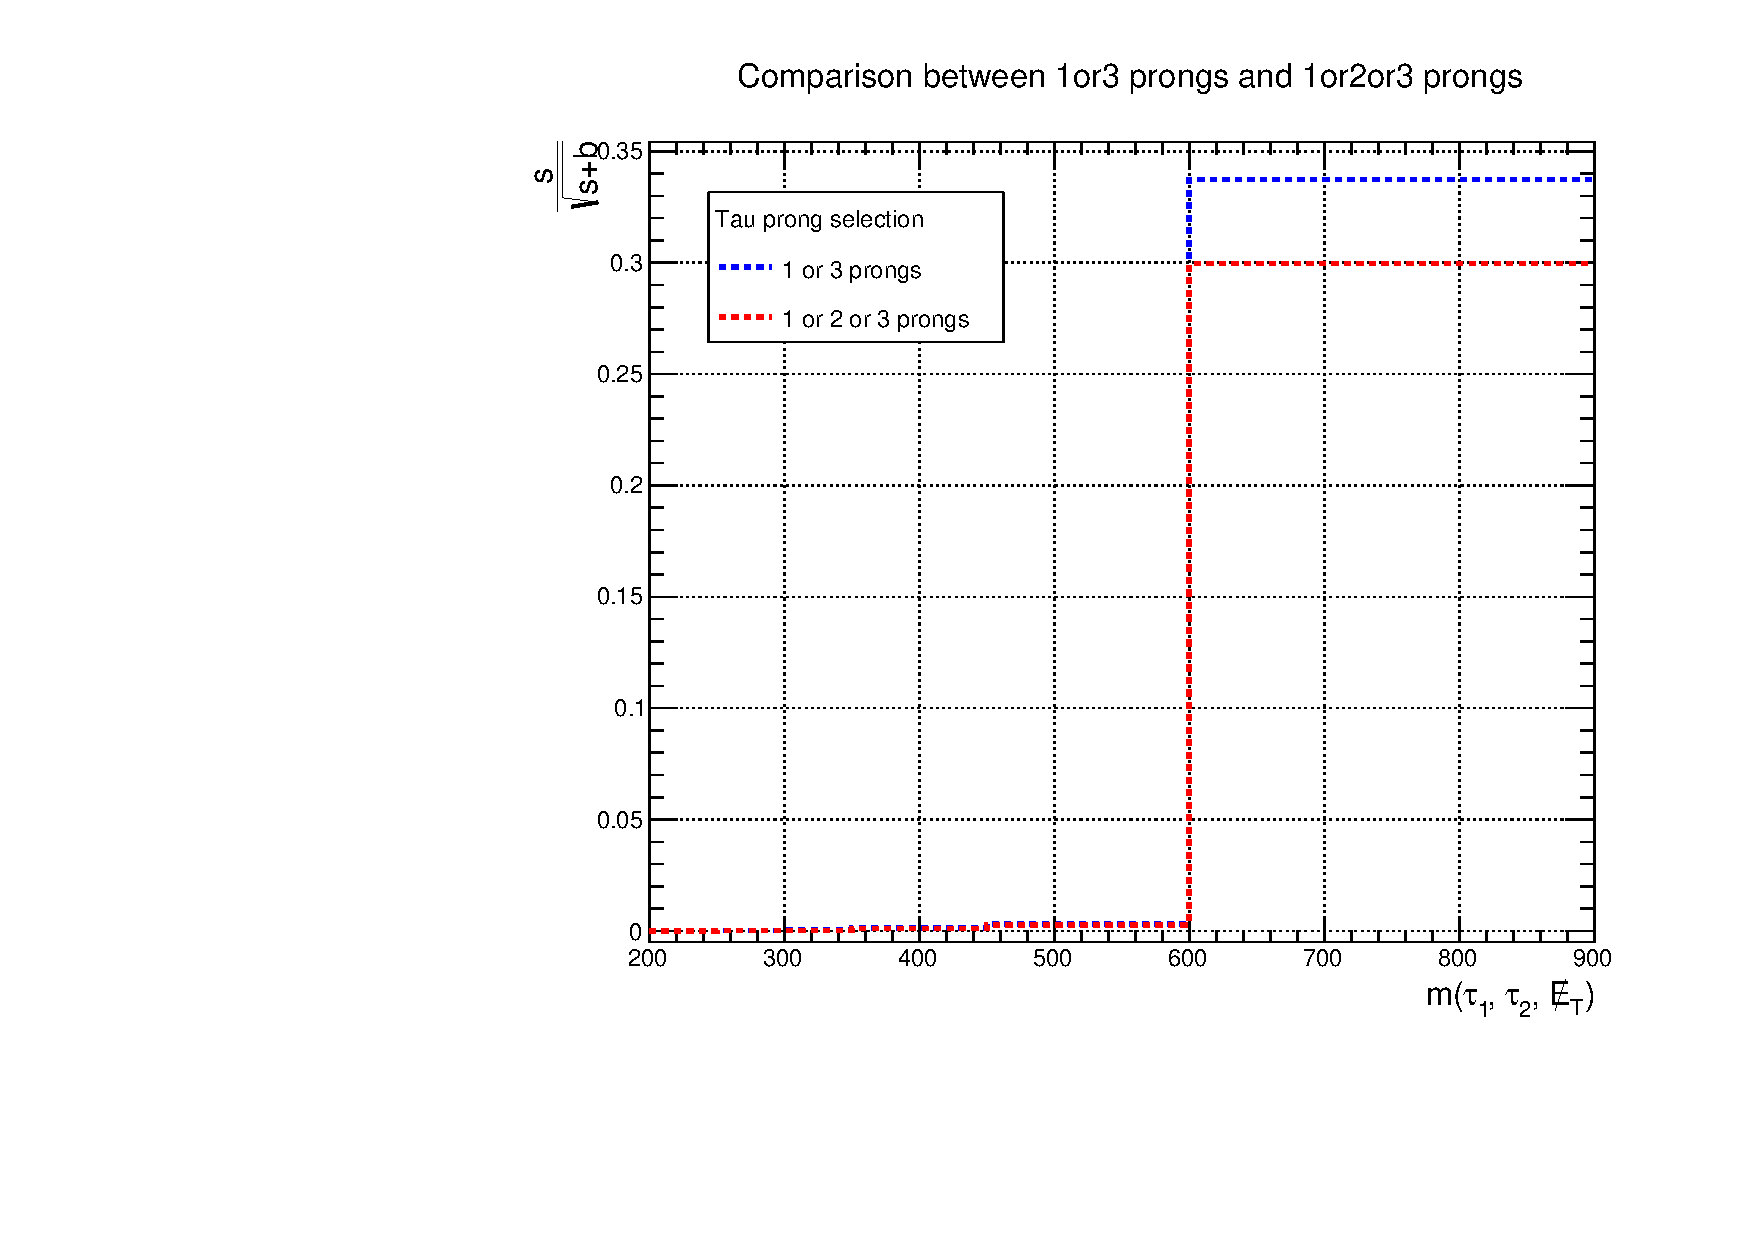
\includegraphics[clip,width=0.5\textwidth]{figuras/AppendiceB/2prongs/prongsComparison.pdf}
 \caption{Significance, as a function of the effective visible mass, obtained 
 with 1or3 prongs (blue) and 1or2or3 prongs (red). \label{fig:prongsappendix}}
\end{center}
\end{figure}

\section{MVA-based Isolation Discriminator Study}
\label{Results:TauID-isoDicr}

\noindent The purpose of the MVA-based isolation discriminator is to reduce the QCD background
contamination. As mentioned in section \ref{subsubsec:IsoDiscriminators}, the energy 
deposits, excluding those coming from the tau decay products, within the isolation cone
define three working points (\textit{loose}, \textit{medium} and \textit{tight}). Less 
energy deposits represents a better discrimination against QCD background, since 
a QCD-jet has higher multiplicity of particles with wider energy profile than
the hadronic tau decay. Table \ref{tab:isoappendix} shows the overall yields obtained using 
the three WPs of the isolation discriminator. Figure \ref{fig:isoappendix} shows 
the significance, as a function of the effective visible mass, for each WP. As expected,
the \textit{tight} WP has the highest significance since it reduces considerably the 
contamination from QCD processes, which are the dominant background in this 
analysis. The results are consistent with the TauPOG recommendation (\textit{tight} WP).
% since  while keeping a relative high signal selection.

% ($\sim$60$\%$)

% In this analysis, since the QCD-processes are the dominant background,
% the MVA-based tight discriminator WP was used. 

 \begin{tiny} 
 \begin{table}[ht] 
 \centering{ 
 \begin{tabular}{ | l | r | r | r |} \hline \hline 
 \multicolumn{4}{|c|}{OVERALL YIELDS}  \\ \hline 
 & \textit{tight} &  \textit{medium} &  \textit{loose}  \\ \hline \hline 
 DY         & 131.61   $\pm$   8.64 & 150.65   $\pm$   9.30 & 181.98   $\pm$   10.82 \\ \hline 
 WJets      & 41.91   $\pm$   5.17 & 72.13   $\pm$   6.76 & 136.69   $\pm$   10.62 \\ \hline 
 DiBoson    & 3.73   $\pm$   1.07 & 4.64   $\pm$   1.19 & 5.09   $\pm$   1.24 \\ \hline 
 \ttbar     & 4.39   $\pm$   1.23 & 4.72   $\pm$   1.28 & 6.46   $\pm$   1.50 \\ \hline 
 QCD        & 382.67   $\pm$   24.84 & 957.93   $\pm$   38.85 & 2300.65   $\pm$   58.22 \\ \hline 
 TOTAL BKG  & 564.30   $\pm$   26.86 & 1190.07   $\pm$   40.56 & 2630.88   $\pm$   60.19 \\ \hline 
 \Zprime~(3 \TeV)   & 1.91   $\pm$   0.02 & 2.26   $\pm$   0.02 & 2.59   $\pm$   0.02 \\ \hline  \hline 
 Significance & 0.34 & 0.27 & 0.24 \\ \hline \hline 
 \end{tabular} 
 } 
 \caption{Signal and background yields obtained using the \textit{tight}, \textit{medium} and \textit{loose} WPs for the MVA-based 
 isolation discriminator. The significance was estimated in the region where the signal is expected. 
  (\mass~$>~$600\GeV). \label{tab:isoappendix} }
 \end{table} 
 \end{tiny} 

\begin{figure}[ht]
\begin{center}
\captionsetup[subfloat]{farskip=0pt,captionskip=0.0cm,labelformat=empty}
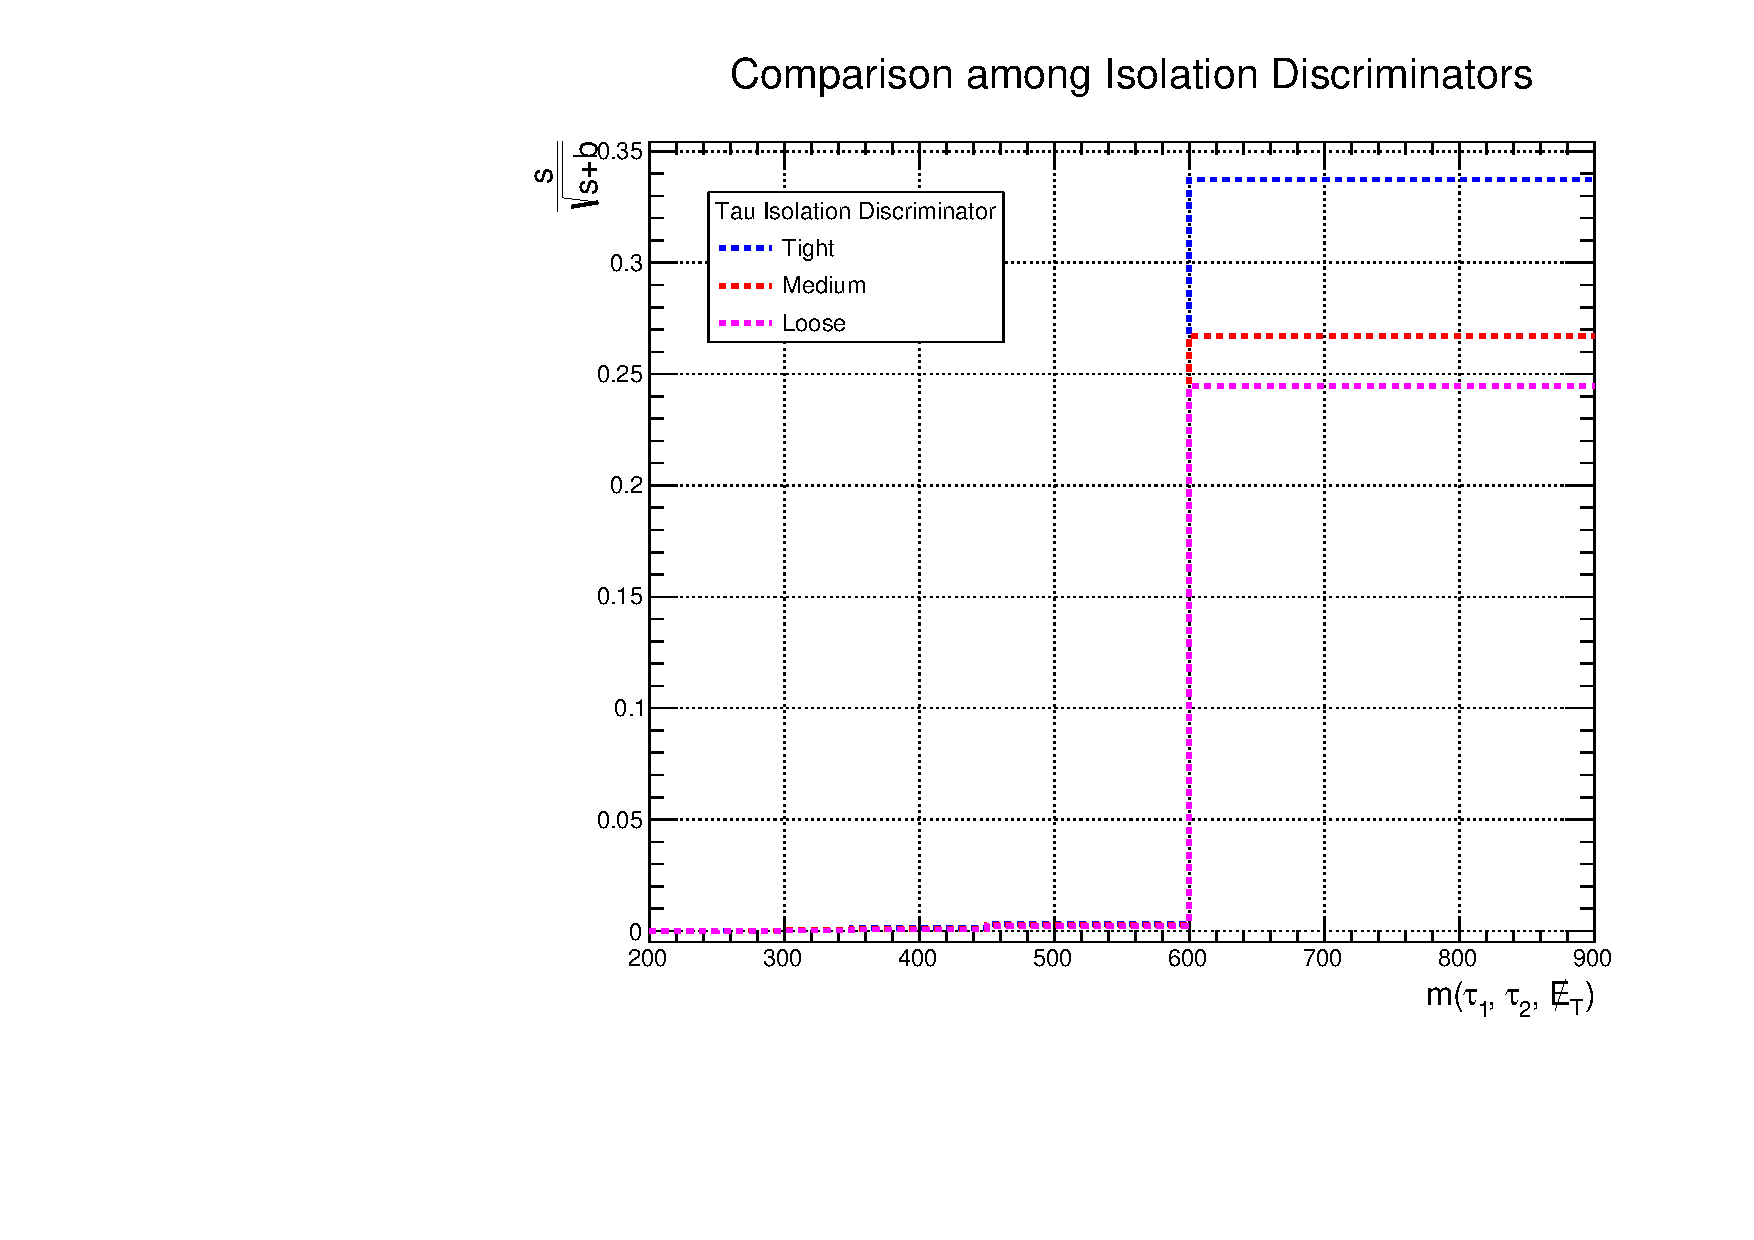
\includegraphics[clip,width=0.5\textwidth]{figuras/AppendiceB/IsoDiscr/IsoDiscrComparison.pdf}
 \caption{Significance, as a function of the effective visible mass, obtained 
 with the \textit{loose} (purple),  \textit{medium} (red) and \textit{tight} (blue) working points of the MVA-based isolation discriminator. \label{fig:isoappendix}}
\end{center}
\end{figure}
\vspace{-1.0cm}

\section{MVA-based against Electron Discriminator Study}
\label{Results:TauID-electronDicr}

\noindent In the case of the MVA-based algorithm developed to discriminate electrons 
from taus, five WP are defined according to the tau identification efficiency and the misidentification rate 
required in each analysis (see Section \ref{subsubsec:DiscriminatorsAgainstElectron}). In this analysis, the 
\textit{loose} WP was used in order to obtain a high tau reconstruction efficiency ($\sim$83$\%$), while keeping 
a relative low misidentification rate ($10^{-2}$). However, the TauPOG recommends to use the \textit{very 
loose} WP since a higher efficiency is achieved ($\sim$85$\%$). Table \ref{tab:electronappendix} shows the overall 
yields obtained using the \textit{loose} and \textit{very loose} WPs of the MVA-based against electron discriminator. As can be noted
in the table, although there are a higher background contribution for the \textit{very loose} WP, the signal 
yield increases due to the higher tau identification efficiency. As a results, the sensitivity of the analysis
is improved using the WP recommended by the TauPOG. Nevertheless, the \textit{loose} WP was used 
in this analysis in order to keep consistency with the \tauh~identification criteria 
% used in the others di-tau channels, in particular with the \taue\tauh~channel. Figure \ref{fig:electronappendix} shows 
used in the others di-tau channels. Figure \ref{fig:electronappendix} shows 
the significance obtained using the \textit{loose} and \textit{very loose} WPs of the MVA-based against electron discriminator.


 \begin{tiny} 
 \begin{table}[ht] 
 \centering{ 
 \begin{tabular}{ | l | r | r |} \hline \hline 
 \multicolumn{3}{|c|}{OVERALL YIELDS} \\ \hline 
 & \textit{loose} &  \textit{very loose}  \\ \hline \hline 
 DY         & 131.61   $\pm$   8.64 & 142.77   $\pm$   9.09 \\ \hline 
 WJets      & 41.91   $\pm$   5.17 & 47.52   $\pm$   5.52 \\ \hline 
 DiBoson    & 3.73   $\pm$   1.07 & 3.76   $\pm$   1.07 \\ \hline 
 \ttbar     & 4.39   $\pm$   1.23 & 5.40   $\pm$   1.37 \\ \hline 
 QCD        & 382.67   $\pm$   24.84 & 400.68   $\pm$   25.35 \\ \hline 
 TOTAL BKG  & 564.30   $\pm$   26.86 & 600.13   $\pm$   27.55 \\ \hline 
 \Zprime~(3 \TeV)   & 1.91   $\pm$   0.02 & 2.19   $\pm$   0.02 \\ \hline  \hline 
 Significance & 0.34 & 0.36 \\ \hline \hline 
 \end{tabular} 
 }
 \caption{Signal and background yields obtained using the \textit{loose} and \textit{very loose} WPs for the MVA-based 
 against electron discriminator. The significance was estimated for 
  \mass~$>~$600\GeV. \label{tab:electronappendix} }
 \end{table} 
 \end{tiny} 
 
%  \textbf{\textcolor{green}{SIGNIFICANCE}} & \textcolor{green}{ 0.34} & \textcolor{green}{ 0.36} \\ \hline  \hline
 
\begin{figure}[ht]
\begin{center}
\captionsetup[subfloat]{farskip=0pt,captionskip=0.0cm,labelformat=empty}
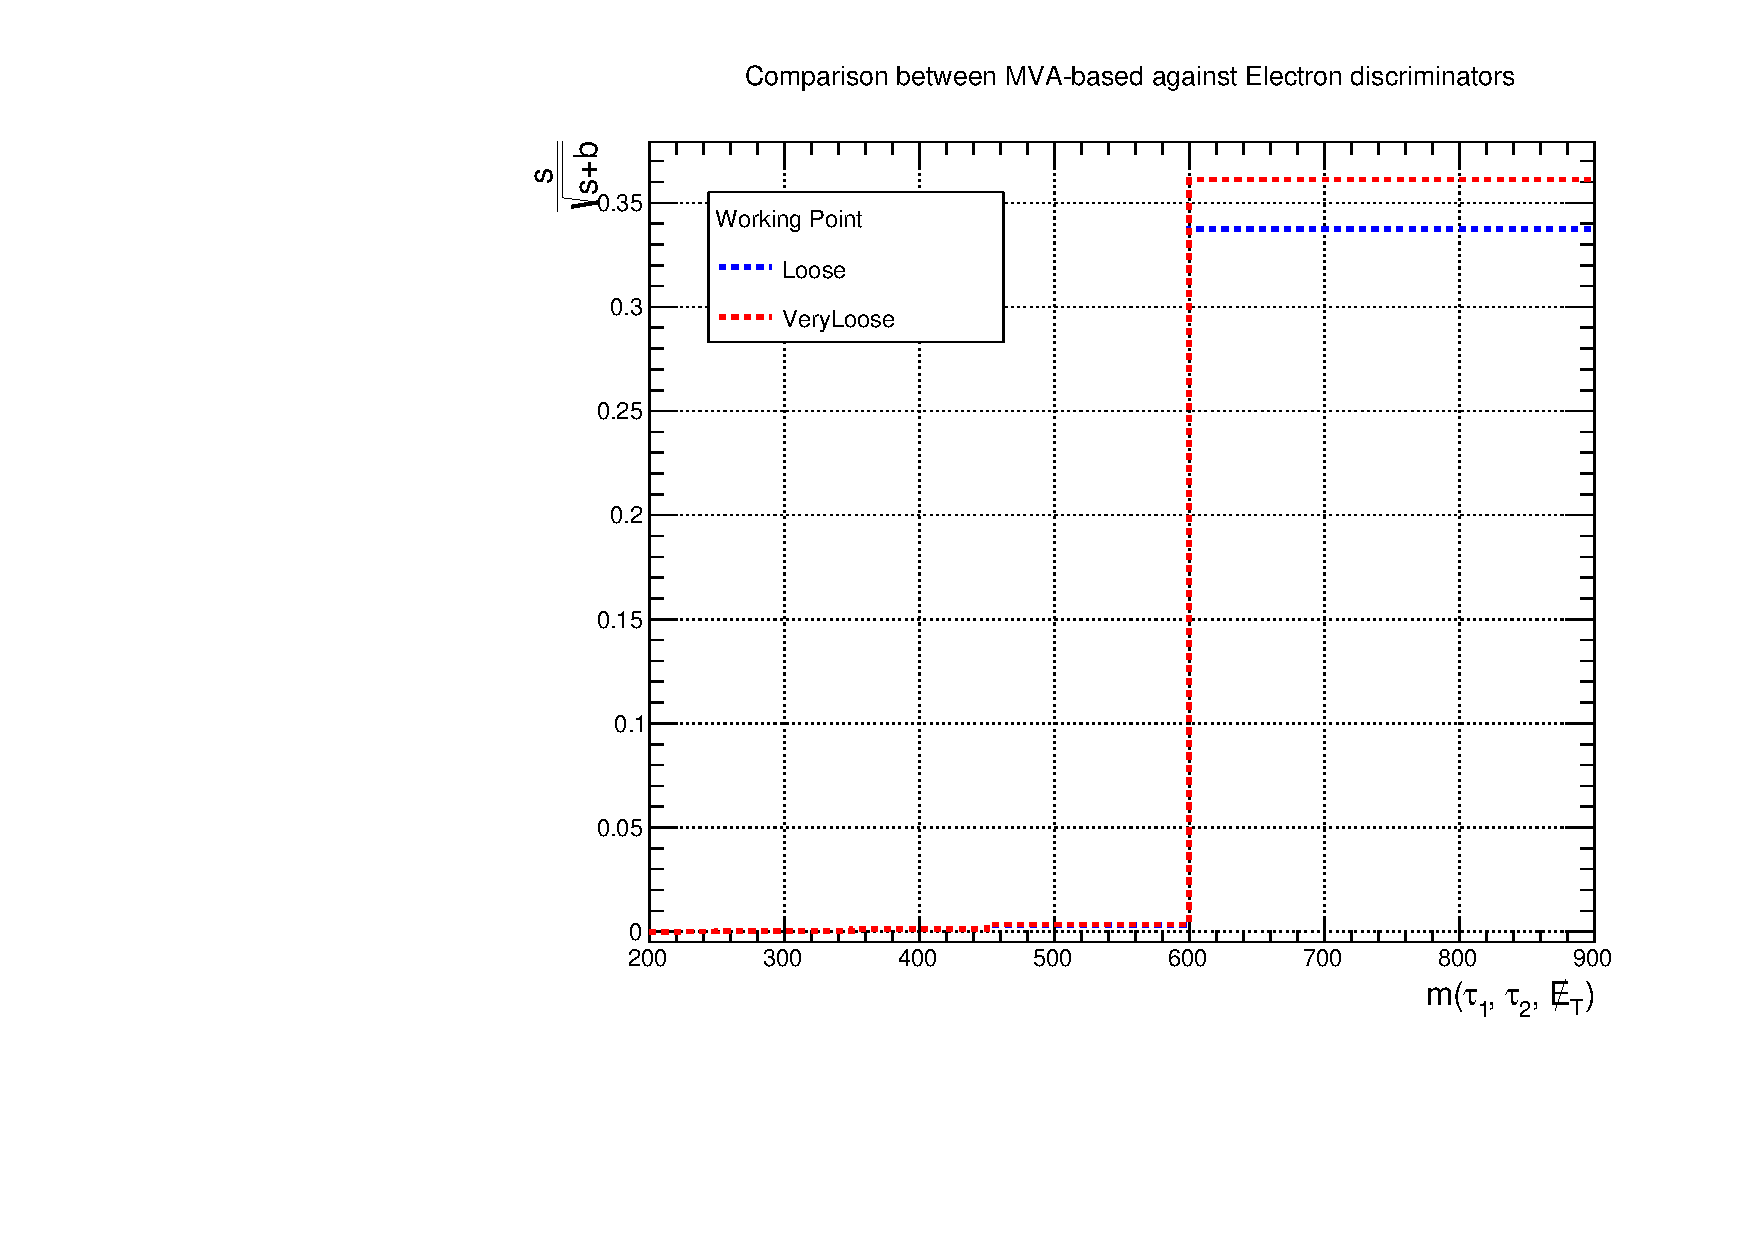
\includegraphics[clip,width=0.5\textwidth]{figuras/AppendiceB/againstElectronWP/againstElectron.pdf}
\caption{Significance, as a function of the effective visible mass, obtained with the 
\textit{loose} (blue) and the \textit{very loose} (red) working points of the MVA-based against electron discriminator. \label{fig:electronappendix}}
\end{center}
\end{figure}


\section{Cutoff-based against Muon Discriminator Study}
\label{Results:TauID-muonDicr}

\noindent Due to the low misidentification rate (of the order of $\sim1 \times 10^{-3}$), the 
working point of the against muon discriminator should not have a considerable 
impact on the sensitivity of the analysis. The \textit{tight}
WP was used in order to be consistent with the other channels. However,
the TauPOG recommends to use the \textit{loose} working point since 
it has a slightly higher tau identification efficiency. Table \ref{tab:muonappendix} shows the overall 
yields obtained using the \textit{tight} and \textit{loose} WPs of the cutoff-based against muon discriminator. The main 
difference between them is the slightly increment on the signal yield obtained 
with the \textit{loose} WP, which is big enough to reach the highest significance. Figure \ref{fig:muonappendix} shows 
the significance obtained using the \textit{tight} and \textit{loose} WPs of the 
cutoff-based against muon discriminator. Although a higher significance is obtained 
with the WP recommended by the TauPOG, the \textit{tight} WP 
was used in this analysis to be consistent with the \tauh~identification criteria 
used in the others di-tau channels.

  \begin{tiny} 
 \begin{table}[ht] 
 \centering{ 
 \begin{tabular}{ | l | r | r |} \hline \hline 
 \multicolumn{3}{|c|}{OVERALL YIELDS} \\ \hline 
 & \textit{tight} &  \textit{loose}  \\ \hline \hline 
 DY         & 131.61   $\pm$   8.64 & 132.84   $\pm$   8.67 \\ \hline 
 WJets      & 41.91   $\pm$   5.17 & 41.94   $\pm$   5.17 \\ \hline 
 DiBoson    & 3.73   $\pm$   1.07 & 3.73   $\pm$   1.07 \\ \hline 
 \ttbar     & 4.39   $\pm$   1.23 & 4.39   $\pm$   1.23 \\ \hline 
 QCD        & 382.67   $\pm$   24.84 & 392.02   $\pm$   25.09 \\ \hline 
 TOTAL BKG  & 564.30   $\pm$   26.86 & 574.91   $\pm$   27.10 \\ \hline 
 \Zprime~(3 \TeV)   & 1.91   $\pm$   0.02 & 1.98   $\pm$   0.02 \\ \hline  \hline 
 \end{tabular} 
 } 
 \caption{Signal and background yields obtained using the \textit{tight} and \textit{loose} WPs for 
 the cutoff-based against muon discriminator. \label{tab:muonappendix} }
 \end{table} 
 \end{tiny} 
%  \textbf{\textcolor{green}{SIGNIFICANCE}} & \textcolor{green}{ 0.34} & \textcolor{green}{ 0.35} \\ \hline  \hline
 
 
\begin{figure}[ht]
\begin{center}
\captionsetup[subfloat]{farskip=0pt,captionskip=0.0cm,labelformat=empty}
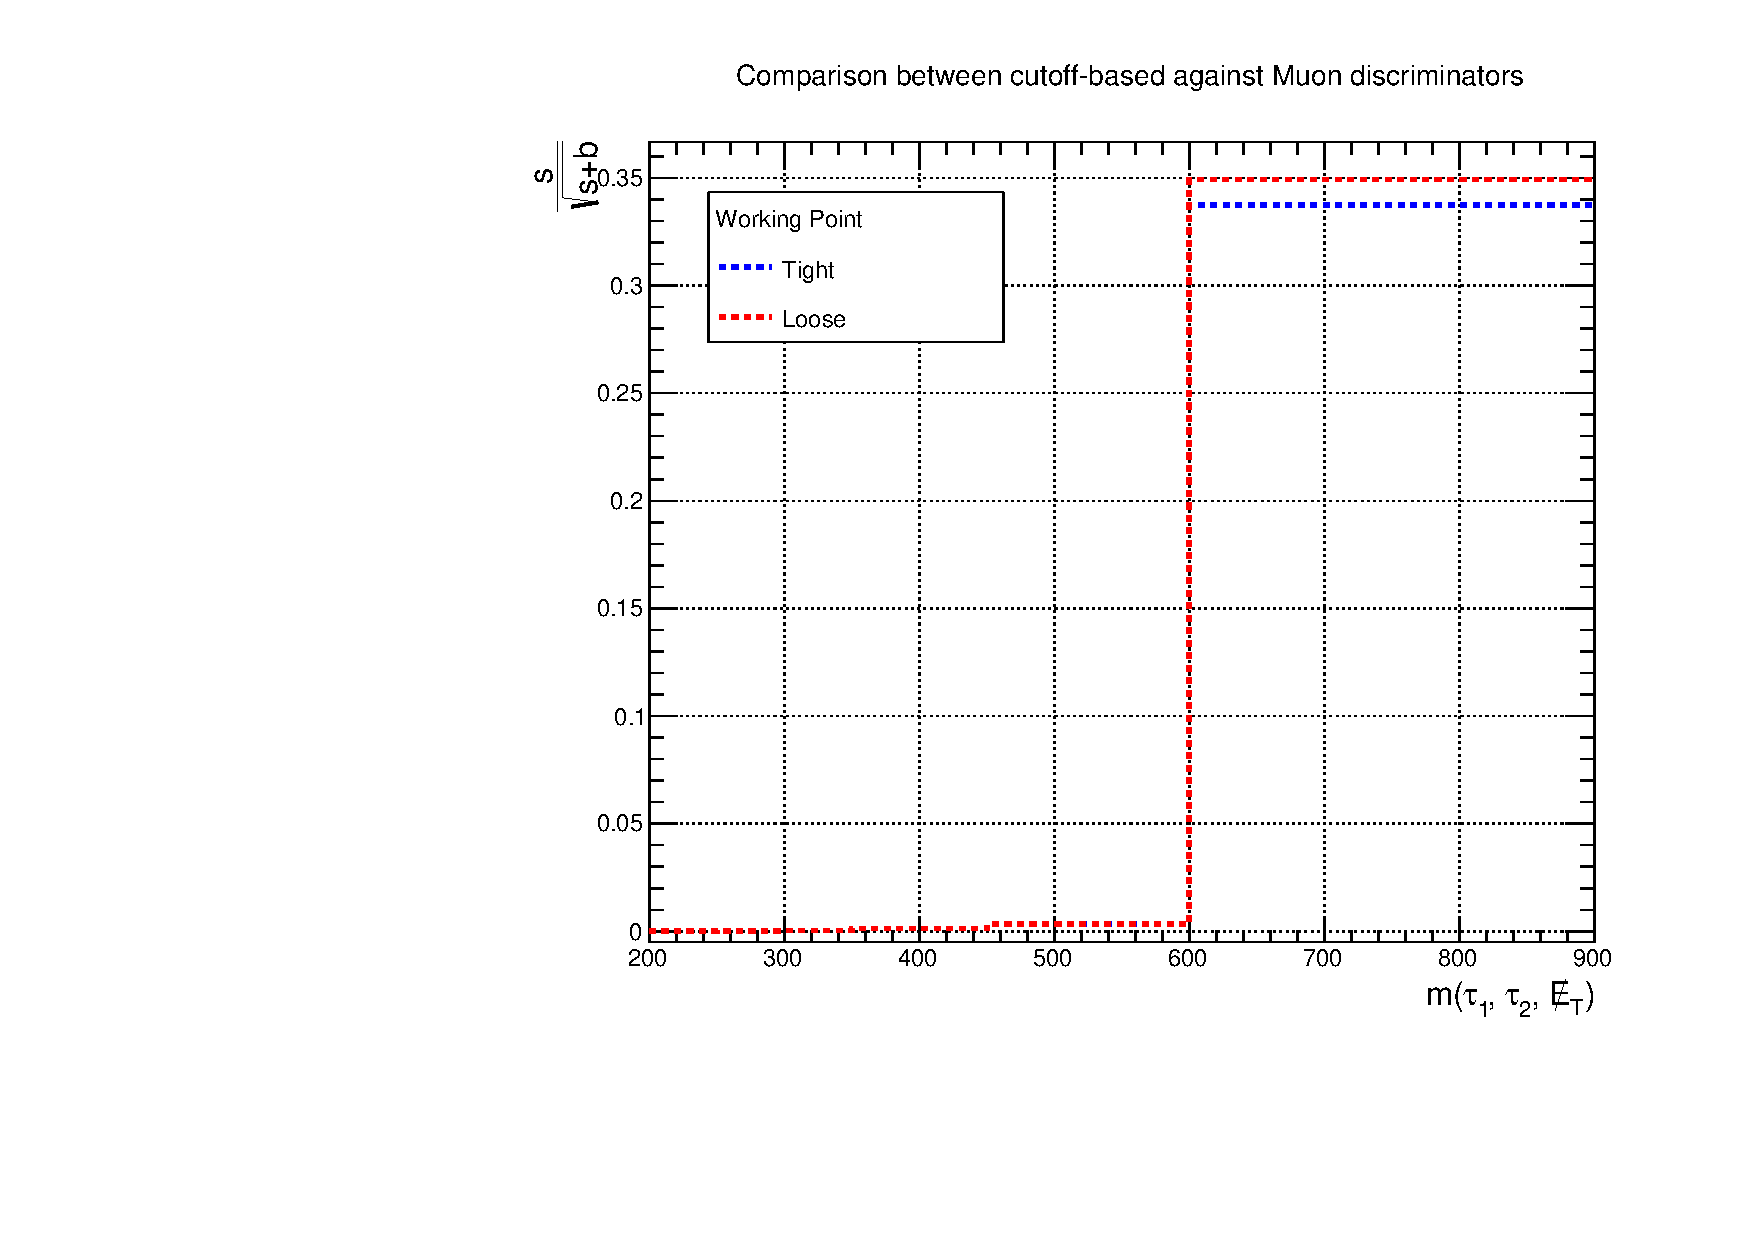
\includegraphics[clip,width=0.5\textwidth]{figuras/AppendiceB/againstMuonWP/againstMuon.pdf}
\caption{Significance, as a function of the effective visible mass, obtained with the 
\textit{tight} (blue) and  \textit{loose} (red) working points of the cutoff-based against muon discriminator. \label{fig:muonappendix}}
\end{center}
\end{figure}

\section{Decay Mode Finding (DMF) Discriminator Study}
\label{Results:TauID-DMFDicr}

\noindent As mentioned in section \ref{subsec:HPS}, there are two versions
of the HPS algorithm in order to reconstruct the tau decay modes: the 
\textit{oldDMF} and the \textit{newDMF}. The \textit{oldDMF} reconstructs only 
the decay modes with 1or3-prongs, while the \textit{newDMF} also considers
the unphysical 2-prong final state. The decay mode discriminator was selected
according to the agreement between data and background in the Drell-Yan control 
region described in section \ref{subsec:DY}. Figure \ref{fig:dmfappendix} shows the 
di-hadronic tau invariant mass distribution in the Drell-Yan control region 
using both decay mode discriminators. As can be noticed, the invariant mass 
shape are consistent with the SM expectation using both discriminators and, therefore,
any of them can be used for the tau identification. The \textit{newDMF} discriminator was used in 
this analysis to be consistent with the other di-tau channels; additionally,
the \textit{newDMF} presents a slightly better bin-by-bin $Data/MC$ agreement. Although the \textit{newDMF} discriminator is not still completely
tested by the collaboration, this work showed that there is not a 
significant impact on the sensitivity of the analysis.

\begin{figure}[ht]
\begin{center}
\captionsetup[subfloat]{farskip=0pt,captionskip=0.0cm,labelformat=empty}
\resizebox{\textwidth}{8.8cm}{
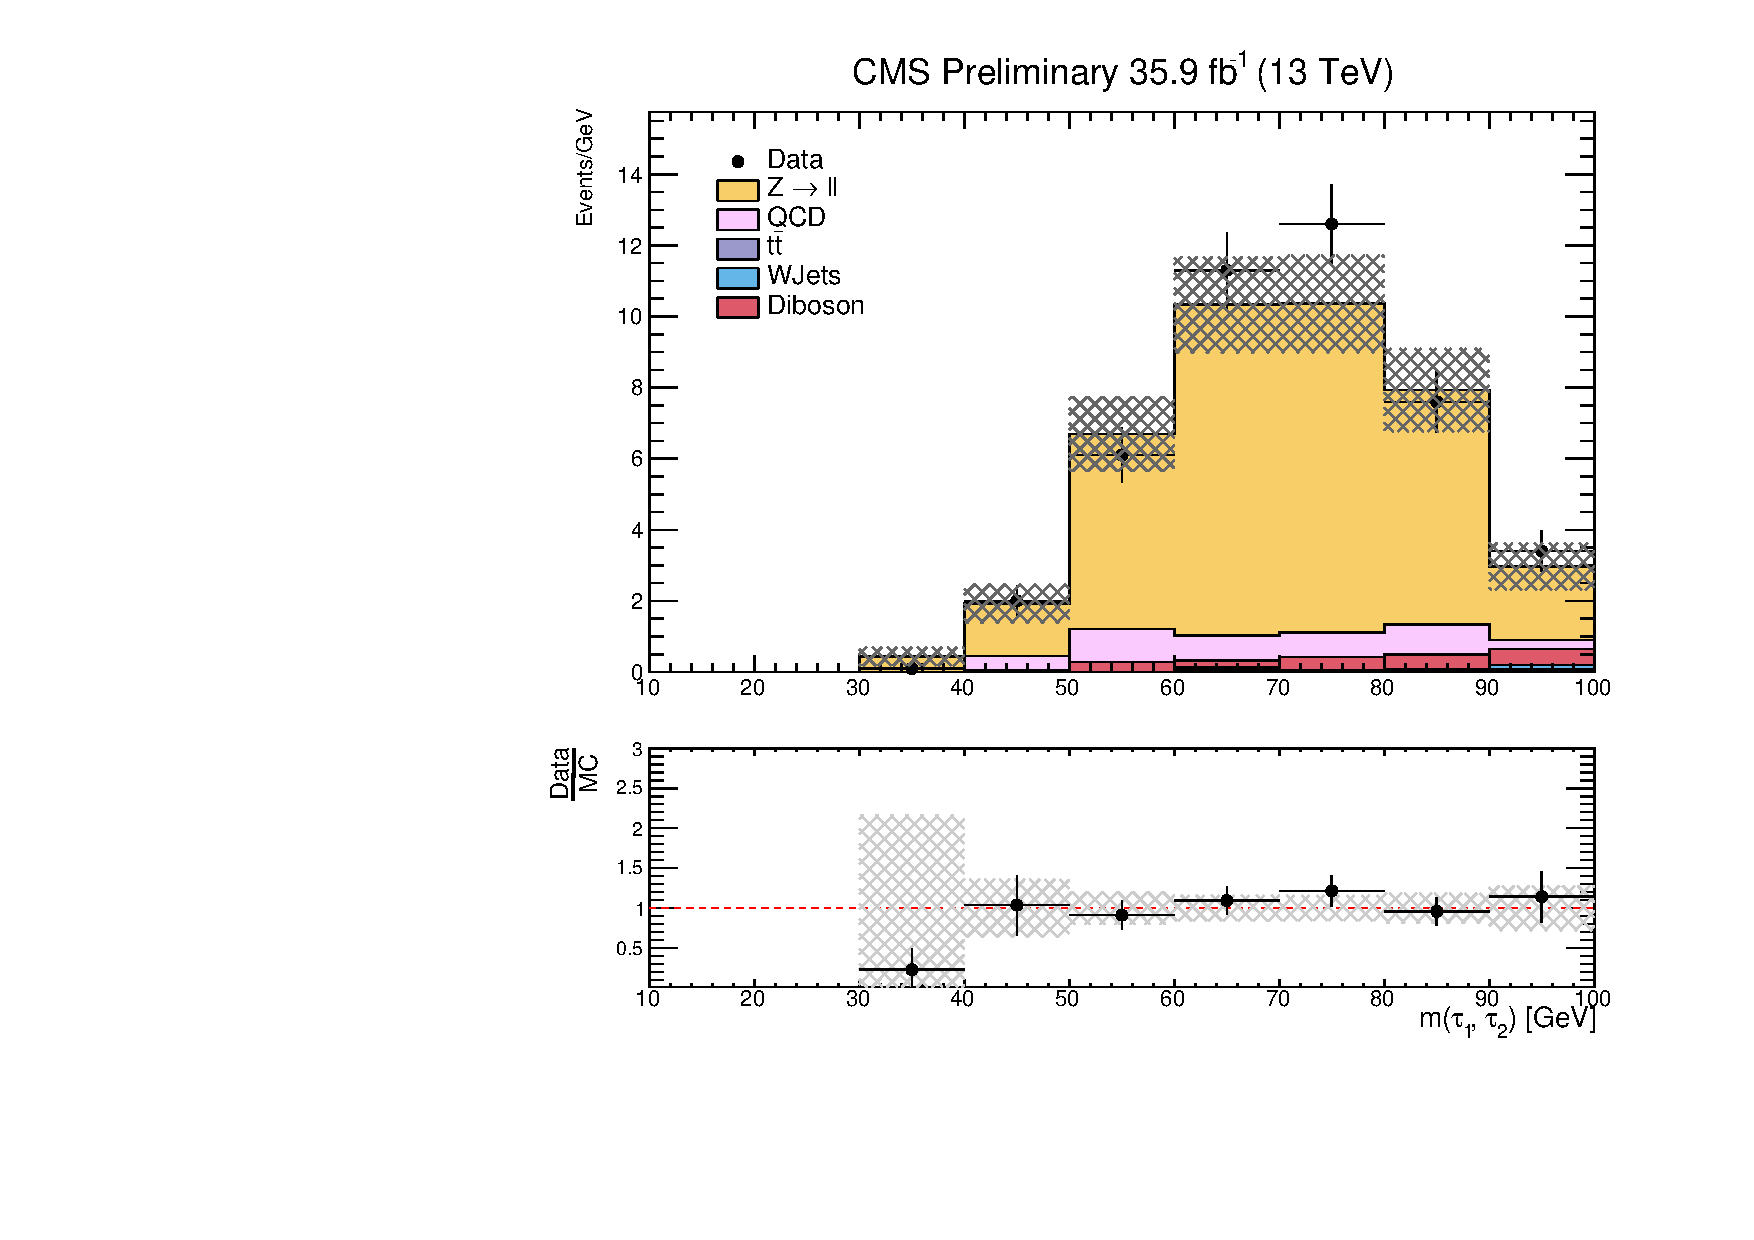
\includegraphics[clip,width=0.46\textwidth]{figuras/AppendiceB/DMF/newDMF.pdf}
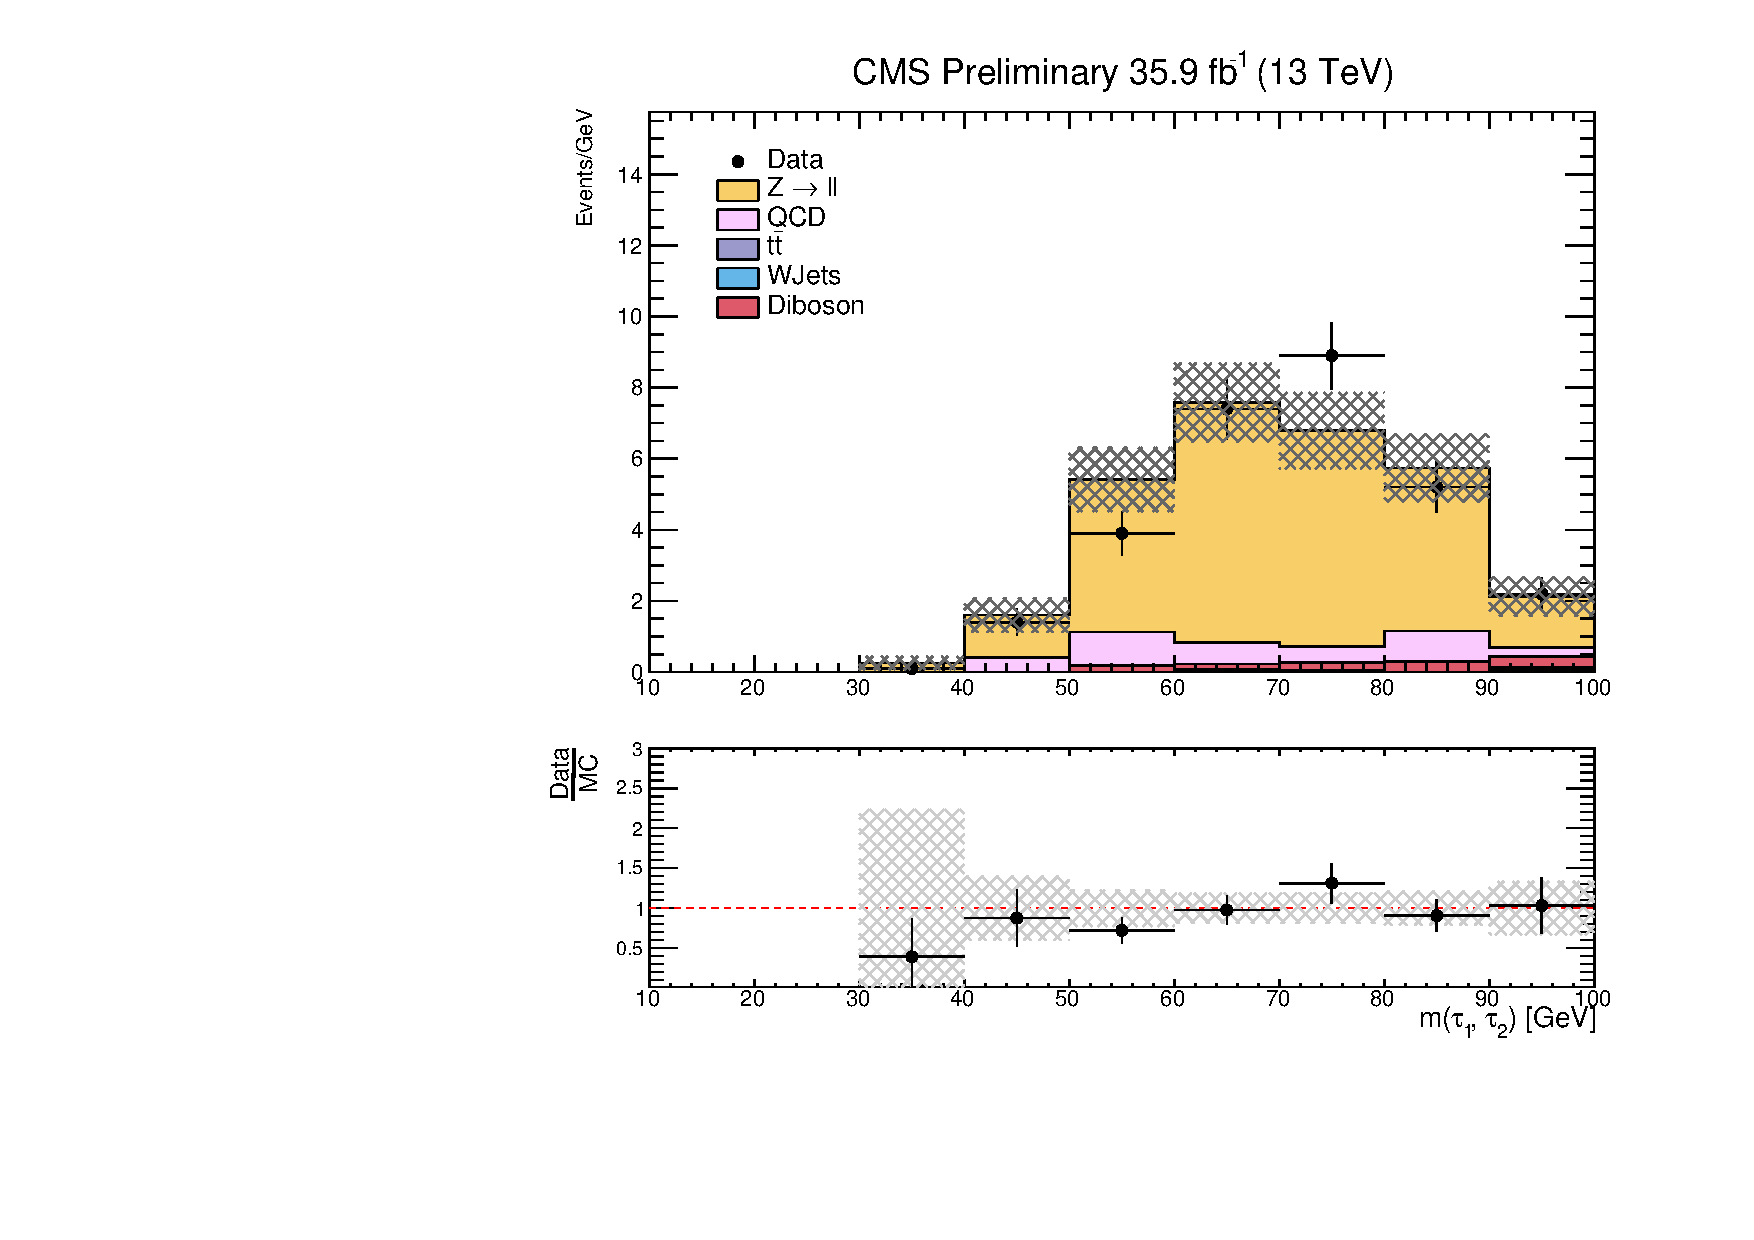
\includegraphics[clip,width=0.46\textwidth]{figuras/AppendiceB/DMF/oldDMF.pdf}
}
\caption{$m(\tau_{h},\tau_{h})$ distribution for the region obtained 
with the \textit{newDMF} (left) and \textit{oldDMF} (right) discriminators in the DY 
selection criteria. Only the statistical uncertainties have been included. \label{fig:dmfappendix}}
\end{center}
\end{figure}

